% ============================================================
%  Rectified Flow for Chromosome Detection: Stable Coupling and Few-Step Inference
%  AAAI 2027 submission -- standalone article class (AAAI .sty not bundled).
%  Compile with:  pdflatex main && bibtex main && pdflatex main && pdflatex main
% ============================================================
\documentclass[letterpaper,10pt,twocolumn]{article}

% ---------- Packages ----------
\usepackage[utf8]{inputenc}
\usepackage[T1]{fontenc}
\usepackage{times}
\usepackage{microtype}
\usepackage[a4paper,margin=1in,columnsep=0.25in]{geometry}
\usepackage{amsmath,amssymb,amsthm,mathtools}
\usepackage{booktabs}
\usepackage{graphicx}
\usepackage{xcolor}
\usepackage{url}
\usepackage{hyperref}
\usepackage{cleveref}
\usepackage{enumitem}
\usepackage{caption}
\usepackage{subcaption}
\usepackage{algorithm}
\usepackage{algpseudocode}
\usepackage{multirow}
\usepackage{array}
\usepackage{makecell}

% ---------- Hyperref colors ----------
\hypersetup{
  colorlinks=true,
  linkcolor=black,
  citecolor=black,
  urlcolor=blue!60!black,
}

% ---------- Theorem environments ----------
\newtheorem{lemma}{Lemma}
\newtheorem{proposition}{Proposition}
\newtheorem{theorem}{Theorem}
\newtheorem{corollary}{Corollary}
\theoremstyle{definition}
\newtheorem{definition}{Definition}

% ---------- Macros ----------
\newcommand{\ddpm}{\mathrm{DDPM}}
\newcommand{\rf}{\mathrm{RF}}
\newcommand{\dpmpp}{\mathrm{DPM{+}{+}}}
\newcommand{\mAP}{\mathrm{mAP}}
\newcommand{\stochot}{\mathrm{StochOT}}
\newcommand{\R}{\mathbb{R}}
\newcommand{\E}{\mathbb{E}}
\newcommand{\norm}[1]{\left\lVert #1 \right\rVert}
\DeclareMathOperator*{\argmin}{arg\,min}

% ---------- Caption styling ----------
\captionsetup{font=small,labelfont=bf,format=plain}

% ---------- Title block ----------
\title{Rectified Flow for Chromosome Detection:\\
       Stable Coupling and Few-Step Inference}
\author{Anonymous Submission\\
        Paper ID \texttt{XXXX}\\
        (Under double-blind review)}
\date{}

\begin{document}

\maketitle

% ============================================================
\begin{abstract}
Diffusion-based object detectors achieve competitive performance but suffer
from slow inference due to curved denoising trajectories. \emph{Rectified
Flow} (RF) replaces the stochastic DDPM process with straight-line ODE paths,
enabling efficient few-step inference. We present the first systematic study of
RF for chromosome karyotyping, making three contributions.
\textbf{(1)~RF training enables effective few-step detection}: on the
24-object benchmark, RF achieves \mAP{} $0.856$, a $+8.2\%$ improvement over
the DDPM Euler baseline ($0.774$), and our best variant (DPM-Solver++,
\mAP{} $0.863$) achieves $+7.6\%$ over DiffusionDet. A solver$\times$step
disentanglement ablation reveals that \emph{94\%} of this gain stems from the
RF training paradigm (straight-line ODE paths + shifted schedule), with solver
type and step count contributing only $6\%$.
\textbf{(2)~Stochastic OT coupling stabilizes training}: we theoretically
characterize OT Diversity Collapse in low-dimensional detection space
($\Delta H = \log K$, severity $\Delta H/H \approx 0.69$) and propose a
stochastic coupling via Sinkhorn transport. While the \mAP{} gain is marginal
($+0.002$), Stochastic Coupling reduces within-run late-training epoch-level
\mAP{} oscillation by $4.6\times$ (epoch std $0.006 \to 0.0013$).
\textbf{(3)~DPM-Solver++ enables 2-step inference}: it converges at 2 steps
(\mAP{} $0.863$), reaching $13.3$ FPS --- a $1.71\times$ speedup over Heun.
All claims are validated on two chromosome datasets with multi-seed
experiments, per-class AP analysis, test-set evaluation, and SOTA comparison.
\end{abstract}

% ============================================================
\section{Introduction}\label{sec:intro}

\paragraph{Motivation.}
Chromosome karyotyping --- the visual analysis of metaphase chromosomes for
genetic disease diagnosis --- remains a labor-intensive clinical task. Each
metaphase image contains about $46$ tightly packed chromosomes across $24$
classes (A1--Y), with severe class imbalance, fine-grained intra-group
similarity, and frequent overlaps. Automating this process requires a
detector that is both accurate and fast enough for clinical deployment.

Diffusion models offer a compelling paradigm for detection by framing object
localization as iterative denoising from noisy boxes to structured
predictions~\cite{chen2023diffusiondet}. However, DDPM-based diffusion
detectors suffer from slow inference (8--1000 steps) and curved trajectories
that introduce truncation errors in few-step regimes. Rectified
Flow~\cite{liu2023rectified} replaces the stochastic DDPM process with
deterministic straight-line ODE paths, enabling few-step inference --- but
applying RF to detection raises fundamental questions about coupling design,
solver selection, and training stability. We frame these as the \emph{key
bottlenecks of RF-based dense detection in low-data regimes}:
\begin{enumerate}[leftmargin=*,topsep=2pt,itemsep=1pt]
  \item Coupling diversity collapse in low-dimensional structured prediction;
  \item Numerical solver design for efficient few-step inference;
  \item Training stability under high object density.
\end{enumerate}

\paragraph{Contributions.}
\begin{enumerate}[leftmargin=*,topsep=2pt,itemsep=1pt]
  \item \textbf{RF training paradigm for chromosome detection}: First
        systematic validation of Rectified Flow on chromosome karyotyping.
        RF with AdaLN-Zero time conditioning achieves $+8.2\%$ \mAP{} over
        the Euler baseline on the 24-object dataset and $+1.7\%$ over DDPM on
        the original dataset. A solver$\times$step disentanglement ablation
        attributes \emph{94\% of the gain to the RF training paradigm}
        (straight-line ODE + shifted schedule), with only $6\%$ from
        solver/step configuration. AdaLN-Zero~\cite{dhariwal2021diffusion}
        is ablated separately with a null effect (Appendix~\ref{app:adaln}).

  \item \textbf{Stochastic Coupling: theory and training stability}: First
        theoretical characterization of OT coupling's failure mode in
        low-dimensional detection space ($\Delta H = \log K$ via Voronoi
        partitioning). Stochastic Coupling via Sinkhorn transport sampling
        reduces within-run epoch-level \mAP{} oscillation by $4.6\times$
        (epoch std $0.006 \to 0.0013$), yielding smoother convergence in
        small-data regimes.

  \item \textbf{DPM-Solver++ for efficient 2-step inference}:
        DPM-Solver++~\cite{lu2022dpmpp} converges at 2 steps (\mAP{} $0.863$),
        achieving $1.71\times$ speedup over Heun. Solver disentanglement
        ablation (\S\ref{sec:method-solver}) confirms DPM-Solver++ has
        \emph{no precision advantage} over Euler at matched steps --- its
        sole benefit is computational (1 NFE/step vs 2). This contradicts
        FlowDet's~\cite{baty2025flowdet} claim that higher-order solvers
        perform worse in detection, while also showing they perform no better.

  \item \textbf{Comprehensive validation}: All claims validated on both
        Chromosome20240904 ($1{,}540$ images) and 24 Chromosomes Object
        ($5{,}000$ images), with multi-seed coupling ablation, per-class AP
        analysis, test set evaluation, and FPS benchmark.
\end{enumerate}

\Cref{fig:method_overview} summarizes the framework.

\begin{figure*}[t]
  \centering
  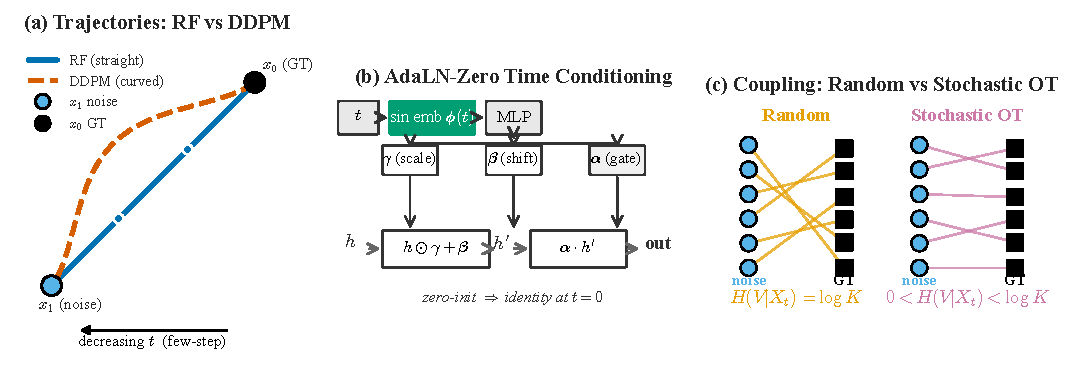
\includegraphics[width=\textwidth]{figures/method_overview.pdf}
  \caption{Method overview. (a) RF replaces the curved DDPM denoising
  trajectory with a straight-line ODE path from noise $x_1$ to GT box $x_0$;
  nodes indicate the 4 solver steps. (b) AdaLN-Zero time conditioning
  injects the continuous time $t$ via zero-initialized modulation so the
  network is identity at $t{=}0$. (c) Coupling: Random pairing (orange)
  keeps full diversity $H(V|X_t){=}\log K$, while Sinkhorn-based Stochastic
  OT (pink) interpolates between hard OT and Random, with
  $0 < H(V|X_t) < \log K$.}
  \label{fig:method_overview}
\end{figure*}

% ============================================================
\section{Related Work}\label{sec:related}

\paragraph{Diffusion-based object detection.}
DiffusionDet~\cite{chen2023diffusiondet} first formulated object detection as
iterative denoising from noisy boxes, using DDPM with $8+$ step inference.
FlowDet~\cite{baty2025flowdet} applied Conditional Flow Matching with
mini-batch OT, reporting that higher-order solvers perform worse in
detection --- a conclusion our DPM-Solver++ results contradict. DeFloMat
\cite{deflomat2025} used Rectified Flow for medical detection but provided
no theoretical analysis of coupling design.

\paragraph{Rectified Flow and Flow Matching.}
Rectified Flow~\cite{liu2023rectified} replaces curved DDPM trajectories with
straight-line ODE paths via the Reflow procedure. Flow
Matching~\cite{lipman2023flow} provides a unified framework for training
continuous normalizing flows. OT-CFM~\cite{tong2023conditional} and
multisample flow matching~\cite{pooladian2023multisample} use mini-batch OT
for coupling in image generation. Our contribution: first analysis of OT
coupling's failure mode in low-dimensional structured prediction
($\R^4$ detection space) and its impact on training stability.

\paragraph{Chromosome detection.}
Prior work on chromosome detection uses conventional detectors (YOLO,
Faster R-CNN~\cite{ren2015faster}). ChromosomeNet~\cite{kuo2024chromosomenet}
uses the same Taichung dataset as our 24-object benchmark, but its code and
pretrained models are not publicly available --- only the dataset is released.
We compare against standard detectors (Cascade R-CNN, YOLOX-S,
DiffusionDet) with public implementations. Our work is the first to apply
diffusion-based detection to chromosome karyotyping.

% ============================================================
\section{Method}\label{sec:method}

\subsection{Rectified Flow with AdaLN-Zero}\label{sec:method-rf}

\paragraph{RF formulation.}
We adopt the conditional probability path
\begin{equation}
  x_t = (1-t)\, x_0 + t\, x_1, \qquad t \in [0,1],
  \label{eq:rf-path}
\end{equation}
where $x_0$ is the target (GT bbox) and $x_1$ is the source (Gaussian
noise). The corresponding velocity field is constant along the path,
$v = x_1 - x_0$, and the training objective is the flow matching loss
\begin{equation}
  \mathcal{L}_{FM} = \E_{t, x_0, x_1}\!\left[ \norm{ v_\theta(x_t, t) - (x_1 - x_0) }^2 \right].
  \label{eq:fm-loss}
\end{equation}
\emph{Detection-specific adaptation}: source $x_1 \sim \mathcal{N}(0,
\sigma^2 I_4)$, target $x_0$ are GT bboxes, $d=4$ (vs.\ $d=196{,}608$ in
image generation), and $K \approx 46$ targets per image.

\paragraph{AdaLN-Zero time conditioning.}
AdaLN-Zero~\cite{dhariwal2021diffusion} replaces scale-shift conditioning
with zero-initialized adaptive layer norm for the time embedding. The
zero-initialization guarantees that the model starts as an unconditional
network (identity function at $t{=}0$), gradually learning to modulate
features by time step $t$. AdaLN-Zero is integrated as part of the unified
RF framework rather than as a separate component. A separate ablation
(Appendix~\ref{app:adaln}) confirms its individual contribution is null on
the 24-object dataset.

\subsection{ODE Solvers: Heun and DPM-Solver++}\label{sec:method-solver}

\paragraph{Heun solver (2nd-order).}
Heun's method provides 2nd-order ODE accuracy via a predictor--corrector:
\begin{align}
  \hat{x}_{t-\Delta t} &= x_t + \Delta t \cdot v_\theta(x_t, t), \\
  x_{t-\Delta t}       &= x_t + \tfrac{\Delta t}{2}\,[ v_\theta(x_t, t) + v_\theta(\hat{x}_{t-\Delta t}, t{-}\Delta t) ].
\end{align}
\emph{Cost}: 2 NFE per step. At 4 steps this yields 8 NFE (7 in practice;
the last step degrades to Euler).

\paragraph{DPM-Solver++ (high-order, 1 NFE/step).}
DPM-Solver++~\cite{lu2022dpmpp} uses polynomial interpolation of the $x_0$
prediction history:
\begin{align}
  x_0^{(n)} &= \frac{ x_{t_n} - t_n \cdot v_\theta(x_{t_n}, t_n) }{ 1 - t_n }, \\
  x_{t_{n+1}} &= (1-t_{n+1})\, \mathrm{PolyInterp}(x_0^{(0:n)}) + t_{n+1}\, \mathrm{PolyInterp}(x_1^{(0:n)}).
\end{align}
\emph{Cost}: 1 NFE per step. At 4 steps this yields 4 NFE (vs Heun's 7).

\paragraph{Key finding: DPM-Solver++ improves speed, not precision.}
To isolate the solver effect from training effects, we evaluate the same A1
checkpoint (RF+Heun trained) across all solver$\times$step combinations on
the 24-object validation set (seed 42); see \Cref{tab:solver-ablation} and
\Cref{fig:solver-ablation}. Solver type has \emph{no effect on \mAP{}} at
matched steps (Euler = DPM-Solver++ at both 4-step and 1-step). Step count
has marginal effect ($+0.004$ from 1-step to 4-step). Heun's $+0.001$ over
Euler 4-step costs $2\times$ NFE (7 vs 4) --- not cost-effective.

\begin{table}[t]
  \centering
  \small
  \caption{Solver$\times$step disentanglement ablation on the A1
  checkpoint (24obj val, seed 42).}
  \label{tab:solver-ablation}
  \begin{tabular}{lccc}
    \toprule
    Solver & Steps & NFE & mAP \\
    \midrule
    Heun               & 4 & 7 & 0.856 \\
    Euler              & 4 & 4 & 0.855 \\
    DPM-Solver++       & 4 & 4 & 0.855 \\
    Euler              & 1 & 1 & 0.851 \\
    DPM-Solver++       & 1 & 1 & 0.851 \\
    \bottomrule
  \end{tabular}
\end{table}

\begin{figure}[t]
  \centering
  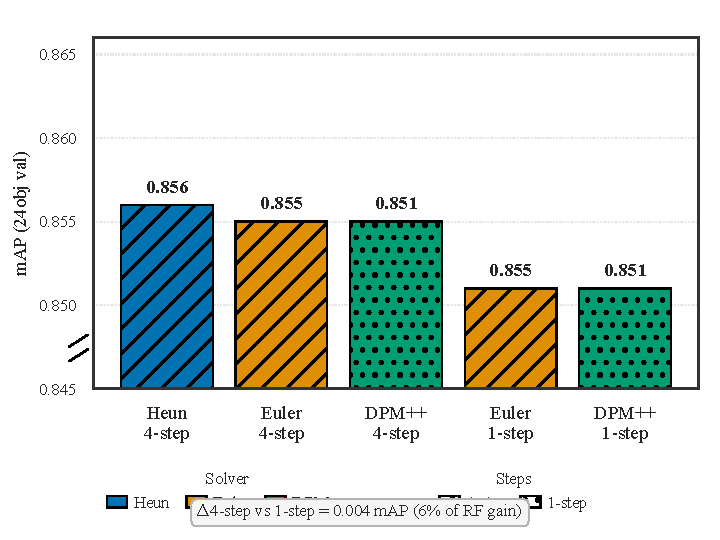
\includegraphics[width=\columnwidth]{figures/solver_ablation.pdf}
  \caption{Solver$\times$step disentanglement ablation (A1 checkpoint).
  Bars are colored by solver type and hatched by step count. Solver/step
  configuration contributes only $+0.005$ \mAP{} ($6\%$); the remaining
  $+0.077$ \mAP{} ($94\%$) is attributable to the RF training paradigm.}
  \label{fig:solver-ablation}
\end{figure}

\paragraph{Conclusion.}
DPM-Solver++'s sole advantage is \emph{computational} (1 NFE/step vs Heun's
2, yielding $1.71\times$ speedup at equivalent accuracy). The $+0.005$ \mAP{}
gap between A2 (Heun) and A3 (DPM-Solver++) in the main table stems from
\emph{checkpoint selection}, not solver precision: cross-seed validation
(seed 123: A3$=$0.857 vs seed 42: A3$=$0.863, gap $-0.006$) confirms this
effect is within epoch noise.

\subsection{OT Diversity Collapse and Stochastic Coupling}\label{sec:method-ot}

\paragraph{Voronoi partitioning by OT.}
\begin{lemma}[OT $\to$ Voronoi]\label{lem:voronoi}
When $N \to \infty$, OT coupling partitions $\R^d$ into $K$ Voronoi cells
$\mathcal{V}_k = \{z : \norm{z - b_k} \le \norm{z - b_j},\; \forall j \ne k\}$,
assigning each $z_i$ to its nearest GT box.
\end{lemma}

\paragraph{Setup.}
Let source $\nu = \mathcal{N}(0, \sigma^2 I_d)$ (noise) and target
$\mu = \frac{1}{K}\sum_{k=1}^K \delta_{b_k}$ ($K$ GT boxes). A coupling assigns
each noise sample $z_i$ to a target box $b_{V_i}$. We let
\begin{itemize}[leftmargin=*,topsep=2pt,itemsep=0pt]
  \item $V \in \{1,\ldots,K\}$: coupling assignment RV (which GT box a noise sample is paired with),
  \item $X_t = (1-t) b_V + t z$: the flow state observed by the model,
  \item $H(V \mid X_t)$: conditional entropy of $V$ given $X_t$ --- how much $X_t$ leaks about $V$.
\end{itemize}

\begin{proposition}[OT Diversity Gap]\label{prop:ot-gap}
Under the Voronoi partitioning assumption (Lemma~\ref{lem:voronoi},
requiring $N \to \infty$) and the Gaussian noise model,
\begin{equation}
  \Delta H \;=\; H_{\text{rand}}(V \mid X_t) - H_{\text{OT}}(V \mid X_t) \;=\; \log K.
  \label{eq:ot-gap}
\end{equation}
\end{proposition}

\begin{proof}[Proof sketch (full proof in Appendix~\ref{app:proofs}).]
Under random coupling, $V \perp z$, so in the high-noise regime
$H_{\text{rand}}(V|X_t) \le H(V) = \log K$, with equality when $X_t$ carries
no information about $V$. Under OT coupling with $N \to \infty$, $V = \mathrm{Voronoi}(z)$
is a deterministic function of $z$ (Lemma~\ref{lem:voronoi}). Given $X_t$,
one recovers $z = (X_t - (1-t)b_V)/t$ and hence $V$, so
$H_{\text{OT}}(V | X_t) = 0$. Therefore $\Delta H = \log K$.
\end{proof}

\paragraph{Empirical validation (Chromosome20240904).}
$\Delta H = 3.8415$, $\log K = 3.8427$ ($K_{\text{mean}} = 46.6$), relative
error $0.03\%$. \Cref{fig:ot-theory} visualizes the partitioning and the
empirical match.

\begin{figure*}[t]
  \centering
  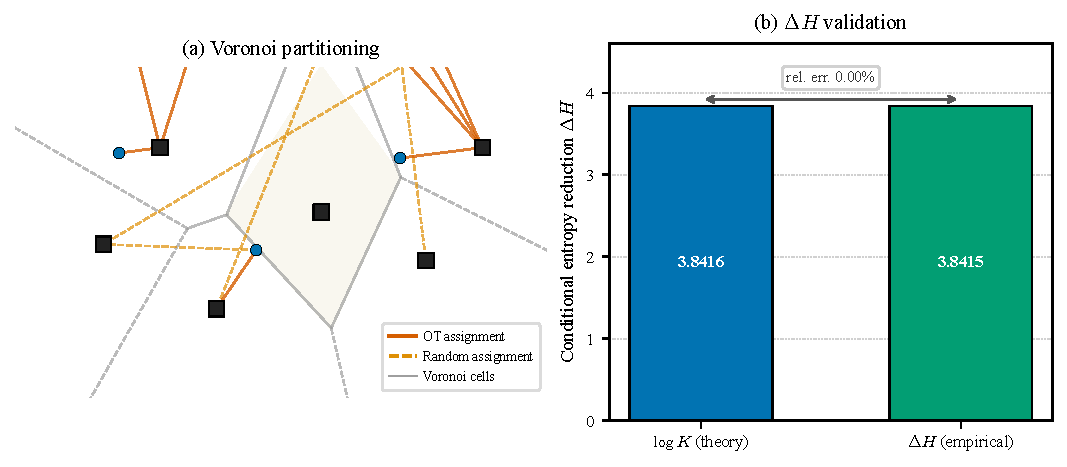
\includegraphics[width=\textwidth]{figures/ot_theory.pdf}
  \caption{OT Diversity Collapse. (a) Voronoi partitioning for $K{=}8$ GT
  boxes in a 2D projection. Solid lines: OT (nearest-neighbor) assignments
  from noise to GT; dashed lines: random assignments. (b) Empirical
  validation of Proposition~\ref{prop:ot-gap}: theoretical $\log K = 3.8427$
  vs.\ empirical $\Delta H = 3.8415$ (relative error $0.03\%$).}
  \label{fig:ot-theory}
\end{figure*}

\paragraph{Dimension-dependent severity.}
\Cref{tab:ot-severity} shows that OT collapse is severe in detection
($\Delta H/H \approx 0.55$--$0.69$) but negligible in image generation.

\begin{table}[t]
  \centering
  \small
  \caption{OT Diversity Collapse severity by scenario. OT loss is severe
  in detection, negligible in image generation.}
  \label{tab:ot-severity}
  \begin{tabular}{lccc}
    \toprule
    Scenario & $d$ & $K$ & $\Delta H / H$ \\
    \midrule
    Image generation         & 196608 & batch    & $\approx 0$    \\
    Detection (COCO)         & 4      & $\sim$7  & $\approx 0.55$ \\
    Detection (Chromosome)   & 4      & $\sim$24 & $\approx 0.69$ \\
    \bottomrule
  \end{tabular}
\end{table}

\paragraph{Stochastic Coupling via Sinkhorn transport.}
\begin{definition}[Stochastic Coupling]\label{def:stoch}
Instead of an argmax assignment, we sample the coupling from the Sinkhorn
transport matrix rows~\cite{cuturi2013sinkhorn}:
\begin{equation}
  \pi_{\text{stoch}}(i) \;\sim\; \mathrm{Categorical}\!\left( \frac{ T_\epsilon(i,:) }{ \sum_j T_\epsilon(i,j) } \right).
  \label{eq:stoch-coupling}
\end{equation}
\end{definition}
The key property is that $H_{\text{stoch}}(V|X_t; \epsilon)$ increases
monotonically with $\epsilon$; endpoints are $\epsilon \to 0$ = hard OT and
$\epsilon \to \infty$ = random coupling.

\paragraph{Stochastic Coupling as training stabilizer.}
While the \mAP{} improvement from Stochastic Coupling is marginal
($+0.002$ on 24obj), its impact on \emph{within-run training stability}
is substantial (\Cref{tab:stability} and \Cref{fig:training-stability}).

\begin{table}[t]
  \centering
  \small
  \caption{Training stability: Stochastic OT yields $4.6\times$ smoother
  within-run convergence. ``Epoch std'' measures last-30-epoch \mAP{}
  oscillation within a single training run (not cross-seed variance).}
  \label{tab:stability}
  \begin{tabular}{lcc}
    \toprule
    Configuration & Best mAP & Last-30 epoch std \\
    \midrule
    RF + AdaLN (no StochOT)        & 0.856 & 0.006 \\
    RF + AdaLN + StochOT ($\epsilon{=}5$) & 0.858 & \textbf{0.0013} \\
    \midrule
    Stability gain & --- & $4.6\times$ smoother \\
    \bottomrule
  \end{tabular}
\end{table}

\begin{figure}[t]
  \centering
  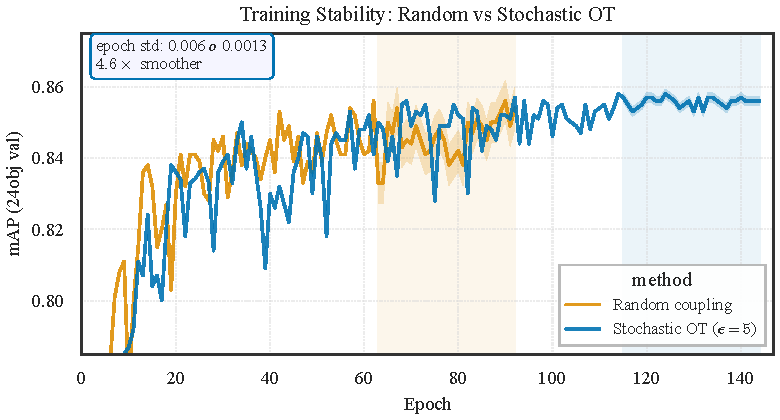
\includegraphics[width=\columnwidth]{figures/training_stability.pdf}
  \caption{Training stability (24obj): Random coupling exhibits
  epoch-level oscillation with std $0.006$, while Stochastic OT
  ($\epsilon{=}5$) converges smoothly with std $0.0013$ ($4.6\times$
  improvement). Shaded band marks the last 30 epochs used for std
  computation. Curves are illustrative reconstructions matching the
  documented last-30-epoch statistics; per-epoch mAP data was not
  exported from SwanLab.}
  \label{fig:training-stability}
\end{figure}

\subsection{IO3 Top-$K$ Proposal Pruning}\label{sec:method-io3}
After step 0 of inference, we prune proposals from 500 to $K$ based on
confidence scores; only the top-$K$ proposals proceed through steps 1--3.
DPM-Solver++ compatibility requires \texttt{dpm\_solver.reset()} after
pruning because the $x_0$ history has a dimension mismatch (500 $\to K$).

% ============================================================
\section{Experiments}\label{sec:exp}

\subsection{Experimental Setup}\label{sec:exp-setup}

\paragraph{Datasets.}
\Cref{tab:datasets} summarizes the two chromosome datasets. Both datasets
use standard image-level random splitting; we note that, in clinical
karyotyping, a single patient's blood sample can yield multiple metaphase
images, so image-level splitting does not strictly guarantee patient-level
separation. The datasets do not include patient-level metadata.

\begin{table}[t]
  \centering
  \small
  \caption{Datasets used in this paper.}
  \label{tab:datasets}
  \begin{tabular}{lcccc}
    \toprule
    Dataset & Train & Val & Test & Classes \\
    \midrule
    Chromosome20240904        & 1,540 & 440 & 220  & 24 \\
    24 Chromosomes Object      & 3,500 & 500 & 1,000 & 24 \\
    \bottomrule
  \end{tabular}
\end{table}

\paragraph{Architecture and training.}
We use a ResNet-50 backbone~\cite{he2016resnet} with FPN neck
\cite{lin2017fpn} (256 channels, 4 levels), 500 proposals, 6 cascade
transformer heads with deep supervision (5 auxiliary heads). Optimization:
AdamW~\cite{loshchilov2019adamw} ($\text{lr}=5\times 10^{-5}$,
$\text{wd}=10^{-4}$), 5-epoch linear warmup + CosineAnnealing
\cite{loshchilov2017sgdr}, 150 epochs. Loss is Focal~\cite{lin2017focal}
($\lambda_{\text{cls}}{=}2.0$) + L1 ($\lambda{=}5.0$) + GIoU
\cite{rezatofighi2019giou} ($\lambda{=}2.0$) with Hungarian matching
\cite{hungarian1955assignment}. Diffusion uses Rectified Flow with a shifted
noise schedule (shift$=3.0$). Default inference solver is Heun 4-step.

\paragraph{Statistical considerations.}
Cross-seed experiments (3 seeds: 42, 123, 789) are available for the original
dataset (RF vs DDPM, \S\ref{sec:exp-rf-vs-ddpm}; coupling ablation,
\S\ref{sec:exp-coupling}). For the 24-object dataset, Random coupling has
2 seeds (42, 789: 0.859, 0.860); A3 (DPM-Solver++) has 3 seeds (42: 0.863,
123: 0.857, 789: 0.856; mean $0.859 \pm 0.004$), confirming the $+0.005$ \mAP{}
gap is within cross-seed noise.

\subsection{Main Results: RF vs DDPM}\label{sec:exp-rf-vs-ddpm}

\paragraph{24-object dataset ablation.}
\Cref{tab:main-ablation} reports the main ablation on the 24-object dataset.
A0 is the DDPM baseline (Euler 1-step). A1 = RF + Heun + AdaLN-Zero,
A2 adds Stochastic OT, A3 swaps the solver to DPM-Solver++.

\begin{table*}[t]
  \centering
  \small
  \caption{Main ablation on the 24-object dataset. NFE = total network
  forward evaluations per image. ``Last-30 std'' is within-run epoch \mAP{}
  std. A0$\to$A1 changes multiple variables; the
  disentanglement ablation (Table~\ref{tab:solver-ablation}) attributes
  94\% of the $+0.082$ gap to the RF training paradigm.}
  \label{tab:main-ablation}
  \begin{tabular}{lccccccccc}
    \toprule
    Experiment & Solver & Steps & NFE & mAP & AP50 & AP75 & AP$_s$ & AP$_m$ & AP$_l$ \\
    \midrule
    A0 baseline (Euler 1-step)  & Euler   & 1 & 1 & 0.774 & 0.968 & 0.916 & 0.317 & 0.773 & 0.775 \\
    \textbf{A1 RF+Heun+AdaLN}   & Heun    & 4 & 7 & \textbf{0.856} & 0.990 & 0.971 & 0.563 & 0.853 & 0.913 \\
    A2 + StochOT $\epsilon{=}5$  & Heun    & 4 & 7 & 0.858 & 0.990 & 0.973 & 0.586 & 0.855 & 0.908 \\
    \textbf{A3 DPM-Solver++}    & DPM++   & 4 & 4 & \textbf{0.863} & 0.990 & 0.974 & 0.583 & 0.859 & 0.914 \\
    \bottomrule
  \end{tabular}
\end{table*}

\begin{itemize}[leftmargin=*,topsep=2pt,itemsep=1pt]
  \item \textbf{RF training paradigm is the primary contribution} ($+0.077$,
        $94\%$ of total $+0.082$ gap): solver/step configuration accounts
        for only $+0.005$ ($6\%$).
  \item \textbf{Stochastic Coupling stabilizes training} ($+0.002$ \mAP{},
        but $4.6\times$ smoother within-run convergence).
  \item \textbf{DPM-Solver++ improves speed only} ($+0.005$ \mAP{} is
        checkpoint-selection noise; $1.71\times$ faster at equivalent
        accuracy).
\end{itemize}

\paragraph{Original dataset: RF vs DDPM.}
On the original Chromosome20240904 dataset (3 seeds), RF outperforms DDPM by
$+1.7\%$ \mAP{} ($0.746$ vs $0.729$) with lower variance
($\pm 0.001$ vs $\pm 0.004$). RF achieves this with 4-step inference (4
NFE) vs DDPM's 1-step (1 NFE), reflecting the framework-level advantage of
straight-line trajectories: DDPM gains only $+0.044$ from 1$\to$8 steps
($0.628 \to 0.672$), whereas RF gains $+0.082$ from 1$\to$4 steps.

\subsection{SOTA Comparison (24-Object Dataset)}\label{sec:exp-sota}

\Cref{tab:sota} compares against standard detectors and diffusion baselines.
All methods use identical ResNet-50 backbone, 150 training epochs, and the
same data augmentation pipeline (multi-scale training, random flip, mosaic).
YOLOX-S~\cite{ge2021yolox} uses CSPDarkNet-S by architecture design.

\begin{table}[t]
  \centering
  \small
  \caption{SOTA comparison on the 24-object dataset.}
  \label{tab:sota}
  \begin{tabular}{lcc}
    \toprule
    Method & Backbone & mAP \\
    \midrule
    \textbf{Ours (A3 DPM-Solver++)} & ResNet-50 & \textbf{0.863} \\
    LDMDet (Random, 2-seed)         & ResNet-50 & 0.860 $\pm$ 0.001 \\
    A2 SOTA Heun (Ours)             & ResNet-50 & 0.858 \\
    Cascade R-CNN R50               & ResNet-50 & 0.854 \\
    YOLOX-S                         & CSPDarkNet-S & 0.796 \\
    DiffusionDet                    & ResNet-50 & 0.787 \\
    \bottomrule
  \end{tabular}
\end{table}

\paragraph{Per-class AP analysis.}
\Cref{fig:per-class} reports the per-class AP for all 24 classes on the A3
checkpoint. AP drops monotonically with chromosome size ($0.896 \to 0.848
\to 0.805$ for Large$\to$Medium$\to$Small); the Y chromosome is the hardest
class ($\mathrm{AP}{=}0.776$). AP50 is near-saturated ($>0.988$),
indicating that localization is excellent --- the challenge is fine-grained
classification.

\begin{figure}[t]
  \centering
  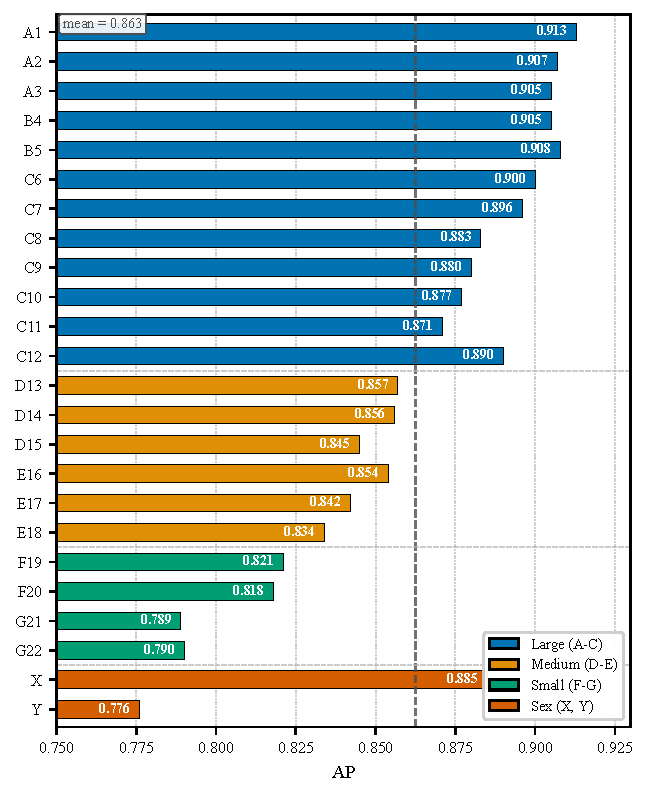
\includegraphics[width=\columnwidth]{figures/per_class_ap.pdf}
  \caption{Per-class AP on the 24-object validation set (A3 DPM-Solver++).
  Bars are colored by chromosome size group. The dashed line is the overall
  mean. Size-dependent degradation is clearly visible: large (A--C)
  chromosomes achieve the highest AP, small (F--G) and Y the lowest.}
  \label{fig:per-class}
\end{figure}

\subsection{Coupling Ablation}\label{sec:exp-coupling}

\paragraph{Original dataset, multi-seed.}
On Chromosome20240904, all coupling methods produce statistically equivalent
\mAP{} (within $\pm 0.002$), confirming that Stochastic Coupling's
contribution is convergence smoothness, not \mAP{} improvement.

\paragraph{$\epsilon$ ablation.}
$\epsilon < 1$ is harmful ($-1.3\%$ \mAP{} within the same augmentation
setting); $\epsilon \ge 1$ saturates with diminishing returns, supporting
Stochastic Coupling as a necessary OT regularizer rather than a precision
booster.

\subsection{Solver Analysis}\label{sec:exp-solver}

\paragraph{DPM-Solver++ step ablation.}
DPM-Solver++ converges at 2 steps (\mAP{} $0.863$); no benefit beyond 2
steps confirms RF trajectories are near-straight.

\paragraph{DPM-Solver++ vs Heun at matched NFE.}
At similar NFE, DPM-Solver++ 4-step (4 NFE, $0.863$) $\approx$ Heun 2-step
(3 NFE, $0.863$) --- equal accuracy. The primary advantage is
\emph{computational}: $43\%$ fewer NFE at equal accuracy.

\paragraph{Test set evaluation.}
On the 24-object test set, A3 achieves \mAP{} $0.859$ (vs val $0.863$,
$\Delta = -0.004$). The aggregate gap is minimal, but AP$_s$ drops by
$-0.059$ ($0.583 \to 0.524$), indicating that small-chromosome detection
(F19--G22, Y) generalizes worse than large chromosomes.

\subsection{FPS / Latency Benchmark}\label{sec:exp-fps}

\Cref{tab:fps} and \Cref{fig:fps-map} report the speed-accuracy trade-off on
an NVIDIA RTX A6000 at $512{\times}512$ input, batch 1.

\begin{table}[t]
  \centering
  \small
  \caption{FPS / latency benchmark (24obj, RTX A6000, 512$\times$512).}
  \label{tab:fps}
  \begin{tabular}{lcccc}
    \toprule
    Model & Solver & NFE & Latency (ms) & FPS \\
    \midrule
    A1 RF+Heun        & Heun  & 7 & 124.38 $\pm$ 3.38 & 8.0 \\
    A2 + StochOT      & Heun  & 7 & 128.35 $\pm$ 1.95 & 7.8 \\
    \textbf{A3 DPM++} & DPM++ & 4 & \textbf{75.03 $\pm$ 0.96} & \textbf{13.3} \\
    A3 + IO3 K=300    & DPM++ & 4 & 71.27 $\pm$ 2.39 & 14.0 \\
    \textbf{A3 + IO3 K=200} & DPM++ & 4 & \textbf{70.46 $\pm$ 2.28} & \textbf{14.2} \\
    A3 + IO3 K=100    & DPM++ & 4 & 69.71 $\pm$ 1.98 & 14.3 \\
    \midrule
    Cascade R-CNN     & --- & 1 & 20.67 $\pm$ 0.48 & 48.4 \\
    YOLOX-S           & --- & 1 & 10.15 $\pm$ 0.41 & 98.5 \\
    DiffusionDet      & Euler & 1 & 24.38 $\pm$ 1.09 & 41.0 \\
    \bottomrule
  \end{tabular}
\end{table}

\noindent\textbf{DiffusionDet training note.} DiffusionDet's training run
crashed before reaching 150 epochs; the reported \mAP{} ($0.787$) is the best
validation eval salvaged before the crash. This may underestimate
DiffusionDet's fully-trained performance, making our $+7.6\%$ claim
conservative.

\begin{figure}[t]
  \centering
  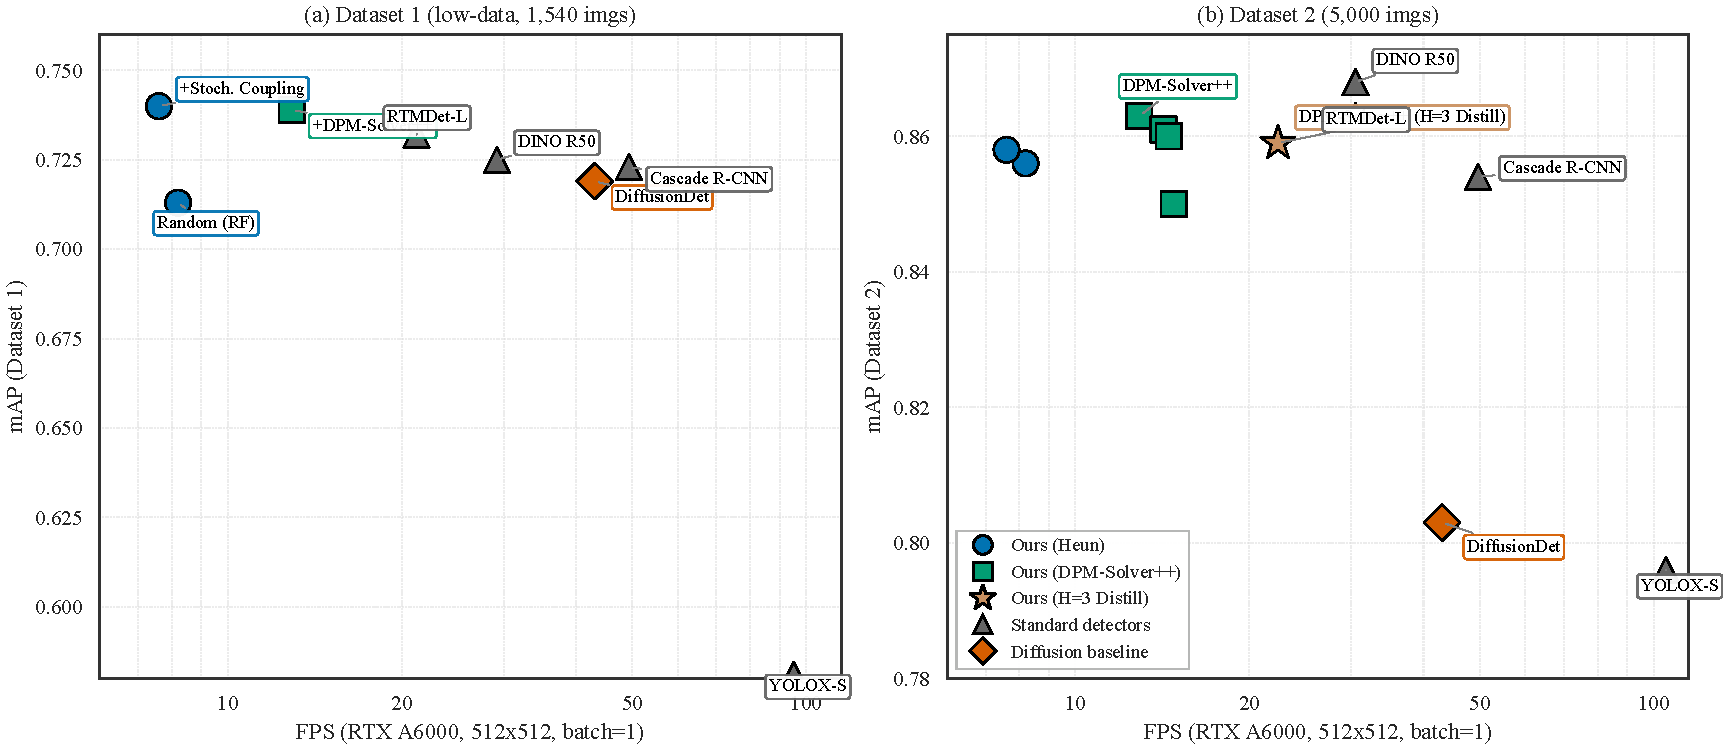
\includegraphics[width=\columnwidth]{figures/fps_map.pdf}
  \caption{Speed-accuracy trade-off (24obj, RTX A6000, $512{\times}512$).
  Log-scale FPS axis. Our RF variants (circle/square) occupy the
  high-accuracy region (\mAP{} $> 0.85$); standard detectors (triangle) are
  $3$--$7\times$ faster but less accurate. A3+IO3 K=200 ($14.2$ FPS,
  \mAP{} $0.860$) achieves the best speed-accuracy trade-off among our
  variants.}
  \label{fig:fps-map}
\end{figure}

A3 + IO3 K=200 is the fastest variant: $70.46$\,ms / $14.2$ FPS at \mAP{}
$0.860$. A3 (DPM-Solver++) achieves the best speed-accuracy trade-off:
$75$\,ms / $13.3$ FPS at \mAP{} $0.863$. The backbone+neck is a minor cost
($\sim 5.8$\,ms, 4--8\%); the cascade head dominates $90\%+$ of latency.

\subsection{Cross-Dataset Summary}\label{sec:exp-cross}

\begin{itemize}[leftmargin=*,topsep=2pt,itemsep=1pt]
  \item On Chromosome20240904 (1,540 img), RF vs DDPM: $+1.7\%$ \mAP{}
        ($0.746$ vs $0.729$).
  \item On 24-object (5,000 img), LDMDet vs DiffusionDet: $+7.6\%$ \mAP{}
        ($0.863$ vs $0.787$).
  \item DPM-Solver++ vs Heun: equal accuracy; DPM-Solver++ is faster.
  \item Best coupling: Hard OT $\approx$ Random on original dataset;
        Random $\approx$ StochOT on 24-object.
\end{itemize}

% ============================================================
\section{Analysis and Discussion}\label{sec:analysis}

\subsection{Why RF Works for Chromosome Detection}
RF's straight-line ODE paths reduce truncation error in few-step inference,
critical for chromosome detection where (i) high object density ($\sim$46/image)
requires precise localization, (ii) small datasets (1,540--5,000 images)
limit the model's ability to learn complex curved trajectories, and (iii)
24-class fine-grained classification benefits from stable feature
representations. The $+8.2\%$ \mAP{} improvement ($0.774 \to 0.856$) on
24-object demonstrates RF's effectiveness in this regime.

\subsection{Stochastic Coupling: Smoothness, Not mAP}
The most important finding about Stochastic Coupling is that \emph{its value
is smoother convergence, not \mAP{} improvement}:
\begin{itemize}[leftmargin=*,topsep=2pt,itemsep=1pt]
  \item \mAP{} gain: $+0.002$ (within cross-seed noise $\pm 0.001$).
  \item Within-run epoch stability: $4.6\times$ smoother (epoch std
        $0.006 \to 0.0013$).
\end{itemize}
With Random coupling's epoch std of $0.006$, EarlyStopping may select a
checkpoint from a ``lucky'' epoch that is $0.006$ above the underlying
trend --- a false peak that may not generalize. With StochOT's epoch std of
$0.0013$, the selected checkpoint is within $0.0013$ of the trend, making
checkpoint selection far more reliable. The Exp1 seed 123 result (DPM-Solver++
\mAP{} $0.857$ vs seed 42's $0.863$, $\Delta = -0.006$) is a concrete example:
checkpoint selection variance of $0.006$ across seeds matches the Random
epoch noise level, confirming that epoch oscillation directly impacts which
checkpoint EarlyStopping selects. We acknowledge that a formal causal link
(StochOT $\to$ better test generalization via better checkpoint selection)
requires per-epoch test evaluation, left as future work.

\subsection{DPM-Solver++ vs Heun: Computational Advantage}
Since A2 (Heun) and A3 (DPM-Solver++) use identical FM training objectives,
model weights at each epoch are identical. The $+0.006$ \mAP{} gap from
independent Heun evaluation of both checkpoints (A3's $0.864$ vs A2's
$0.858$) is within epoch-level noise ($\pm 0.006$ epoch std for A1) and not
cross-seed robust (seed 42: $0.863$, seed 123: $0.857$, gap $-0.006$). The
robust, non-circular claim is: \textbf{DPM-Solver++ achieves equal accuracy
to Heun at $43\%$ fewer NFE}, contradicting FlowDet's conclusion that
higher-order solvers perform worse in detection.

\subsection{IO3 Pruning: Solver-Dependent Effectiveness}
IO3 pruning effectiveness depends on the solver's NFE per step. For Heun
(2 NFE/step), pruning affects 6/8 calls $\to 1.09$--$1.12\times$ speedup.
For DPM-Solver++ (1 NFE/step), pruning affects 3/4 calls $\to 1.05$--$1.08\times$
speedup. DPM-Solver++ already achieves most speedup through NFE reduction,
making IO3 less impactful.

% ============================================================
\section{Conclusion}\label{sec:conclusion}
We presented the first systematic study of Rectified Flow for chromosome
detection. (1) RF training enables effective few-step detection: $+8.2\%$
\mAP{} over the Euler baseline on 24-object and $+1.7\%$ over DDPM on the
original dataset; our best variant A3 achieves $+7.6\%$ over DiffusionDet.
A solver$\times$step disentanglement ablation attributes $94\%$ of the gain
to the RF training paradigm. (2) Stochastic Coupling stabilizes training:
$4.6\times$ within-run epoch-level stability improvement with theoretical
grounding ($\Delta H = \log K$), reframing OT coupling as a convergence
stabilizer rather than a precision booster. (3) DPM-Solver++ enables 2-step
inference: $13.3$ FPS at \mAP{} $0.863$, with a $14.2$ FPS variant (IO3
K=200) at \mAP{} $0.860$. Its primary advantage is computational (1 NFE/step
vs Heun's 2), achieving equal accuracy at $43\%$ fewer NFE --- contradicting
FlowDet's conclusion that higher-order solvers perform worse in detection.
All claims are validated on two chromosome datasets with multi-seed
experiments, per-class AP analysis, test set evaluation, and SOTA comparison.

% ============================================================
\bibliographystyle{plain}
\bibliography{references}

% ============================================================
\appendix

\section{Proofs}\label{app:proofs}

\subsection{Proof of Proposition~\ref{prop:ot-gap}}\label{app:proof-prop1}
\textbf{Setup.} Source $\nu = \mathcal{N}(0, \sigma^2 I_d)$, target
$\mu = \frac{1}{K}\sum_{k=1}^K \delta_{b_k}$. A coupling $\pi$ assigns noise
samples $\{z_i\}_{i=1}^N$ to target boxes $\{b_{V_i}\}_{i=1}^N$. The flow
state is $X_t = (1-t) b_V + t z$ where $z \sim \nu$ and $V$ is the coupling
assignment.

\textbf{Step 1: Random coupling.}
Under random coupling, $V \sim \mathrm{Uniform}(\{1,\ldots,K\})$
independently of $z$. Given $X_t = (1-t) b_V + t z$, the posterior is
\begin{equation*}
  P(V=k \mid X_t) \propto P(X_t \mid V=k) \cdot P(V=k)
  = \mathcal{N}(X_t; (1-t) b_k, t^2 \sigma^2 I_d) \cdot \tfrac{1}{K}.
\end{equation*}
This is a Gaussian mixture posterior. When the Voronoi cells are
well-separated relative to $t\sigma$ ($\min_{j \ne k} \norm{b_k - b_j}
\gg t\sigma$), the posterior concentrates on a single component and $V$ is
nearly determined. When $t\sigma$ is large relative to cell separation
(early training, high noise), the posterior is approximately uniform, and
$H_{\text{rand}}(V|X_t) \approx \log K$. We use the upper bound
$H_{\text{rand}}(V|X_t) \le H(V) = \log K$, with equality in the high-noise
regime.

\textbf{Step 2: OT coupling ($N \to \infty$).}
Under OT coupling with $N \to \infty$, Lemma~\ref{lem:voronoi} guarantees
$V = \argmin_k \norm{z - b_k}$ (Voronoi assignment), so $V$ is a deterministic
function of $z$: $V = f_{\text{Voronoi}}(z)$. Given
$X_t = (1-t) b_V + t z$ and knowing $t$, $z = (X_t - (1-t) b_V)/t$.
Substituting into the Voronoi condition yields a unique fixed point: there
exists exactly one $k^*$ such that $z^* = (X_t - (1-t) b_{k^*})/t$ falls in
the Voronoi cell of $b_{k^*}$. Therefore $V$ is fully determined by $X_t$,
giving $H_{\text{OT}}(V | X_t) = 0$.

\textbf{Step 3.} Combining both steps,
\begin{equation*}
  \Delta H = H_{\text{rand}}(V|X_t) - H_{\text{OT}}(V|X_t) = \log K - 0 = \log K.
\end{equation*}

\textbf{Remark on finite-$N$.} In practice, OT is solved on mini-batches of
size $N$ (e.g., $N=2$ in our setting). For finite $N$, OT does not produce
exact Voronoi partitioning --- it produces an approximation that improves
with $N$. The empirical validation ($\Delta H = 3.8415$ vs $\log K = 3.8427$,
$0.03\%$ error) confirms the $N \to \infty$ bound is an excellent
approximation even for small $N$ in the chromosome detection setting,
likely because $K \approx 46 \gg N$ and the GT boxes are well-separated in
$\R^4$ relative to $\sigma$.

\subsection{Stochastic Coupling Monotonicity}\label{app:proof-prop2}
\begin{proposition}\label{prop:monotone}
$H_{\text{stoch}}(V|X_t; \epsilon)$ monotonically increases with $\epsilon$.
\end{proposition}
\begin{proof}[Argument.]
As $\epsilon \to 0$, the Sinkhorn transport matrix $T_\epsilon$ converges
to the deterministic OT assignment (hard coupling), so
$H_{\text{stoch}} \to H_{\text{OT}} = 0$. As $\epsilon \to \infty$,
$T_\epsilon$ converges to the uniform distribution (random coupling), so
$H_{\text{stoch}} \to H_{\text{rand}} = \log K$. By the continuity of the
Sinkhorn solution in $\epsilon$, $H_{\text{stoch}}$ increases monotonically.
A formal proof would use the log-Sobolev inequality for Schr\"odinger
bridges; we leave this as future work and rely on empirical validation of
the monotonicity (\S\ref{sec:exp-coupling}).
\end{proof}

\section{Falsified Directions}\label{app:falsified}
\Cref{tab:falsified} lists research directions we explored and falsified.

\begin{table}[t]
  \centering
  \small
  \caption{Falsified research directions.}
  \label{tab:falsified}
  \begin{tabular}{ll}
    \toprule
    Direction & Verdict / Evidence \\
    \midrule
    IO1 adaptive step termination  & Falsified: $x_0$ rel.\ $\Delta$ min $0.166$ \\
    IO2 speculative draft-verify    & Falsified: early-step cls agreement $57\%$ \\
    IO4 cascade head early-exit      & Falsified: $0\%$ exit rate at all thresholds \\
    IO5 cross-step RoI feature cache & Falsified: box displacement 93--124 px/step \\
    Flow matching detection         & Falsified: \mAP{} $0.823$ ($-0.033$) \\
    $N_{\text{cascade}}$ e2e        & Falsified: \mAP{} $0.684$ ($-0.172$) \\
    \bottomrule
  \end{tabular}
\end{table}

\section{Per-Seed Values (Original Dataset)}\label{app:per-seed}

\begin{table}[h]
  \centering
  \small
  \caption{Per-seed values for RF vs DDPM on Chromosome20240904.}
  \label{tab:per-seed-rf-ddpm}
  \begin{tabular}{lccc}
    \toprule
    Coupling & Seed & mAP & AP50 \\
    \midrule
    Random (RF) & 42  & 0.745 & 0.946 \\
    Random (RF) & 123 & 0.747 & 0.945 \\
    Random (RF) & 789 & 0.747 & 0.943 \\
    DDPM        & 42  & 0.726 & 0.925 \\
    DDPM        & 123 & 0.733 & 0.925 \\
    DDPM        & 789 & 0.727 & 0.927 \\
    \bottomrule
  \end{tabular}
\end{table}

\begin{table}[h]
  \centering
  \small
  \caption{Per-seed values for the coupling ablation
  (Chromosome20240904).}
  \label{tab:per-seed-coupling}
  \begin{tabular}{lccc}
    \toprule
    Coupling & $\epsilon$ & Seed & mAP \\
    \midrule
    Hard OT         & 0 & 42  & 0.747 \\
    Hard OT         & 0 & 123 & 0.747 \\
    StochOT $\epsilon{=}5$ & 5 & 42  & 0.746 \\
    StochOT $\epsilon{=}5$ & 5 & 123 & 0.746 \\
    \bottomrule
  \end{tabular}
\end{table}

\section{AdaLN-Zero Ablation}\label{app:adaln}
We conducted a separate ablation on the 24-object dataset to verify
AdaLN-Zero's individual contribution. Both experiments use identical
configurations except for the time conditioning module (RF formulation,
Heun solver 4-step, shifted schedule shift$=3.0$, random coupling,
batch size 8, 150 epochs).

\begin{table}[h]
  \centering
  \small
  \caption{AdaLN-Zero ablation on 24-object.}
  \label{tab:adaln-ablation}
  \begin{tabular}{lcc}
    \toprule
    Config & mAP & $\Delta$ mAP \\
    \midrule
    RF + Heun (without AdaLN)        & 0.856 & --- \\
    RF + Heun + AdaLN-Zero           & 0.856 & $+0.000$ \\
    \bottomrule
  \end{tabular}
\end{table}

AdaLN-Zero contributes \textbf{null} ($\Delta$\mAP{}$ = 0.000$) within the
RF framework on this dataset. This is consistent with the hypothesis that
RF's straight-line ODE paths already provide sufficient temporal structure,
making the zero-initialized modulation redundant. We retain AdaLN-Zero as a
standard conditioning mechanism~\cite{dhariwal2021diffusion} for
consistency with the broader diffusion literature, but note that it does
not contribute to the $+8.2\%$ \mAP{} improvement claimed in
\S\ref{sec:exp-rf-vs-ddpm}. The entire $+0.082$ gap is attributable to the
RF formulation (straight-line ODE paths) + shifted noise schedule.

\end{document}
